\subsection{Prototipos}


/watcher
Muestra el perfil de un watcher, en el puedes ver todas las contribuciones de este junto con la lista de visualizaciones que ha creado.
Se permitirá un mínimo de customización. Y se podrá enlazar el perfil de wikipedia


/home
Para usuarios autenticados, les permite ver diferentes secciones relevantes para ellos

\begin{figure}
    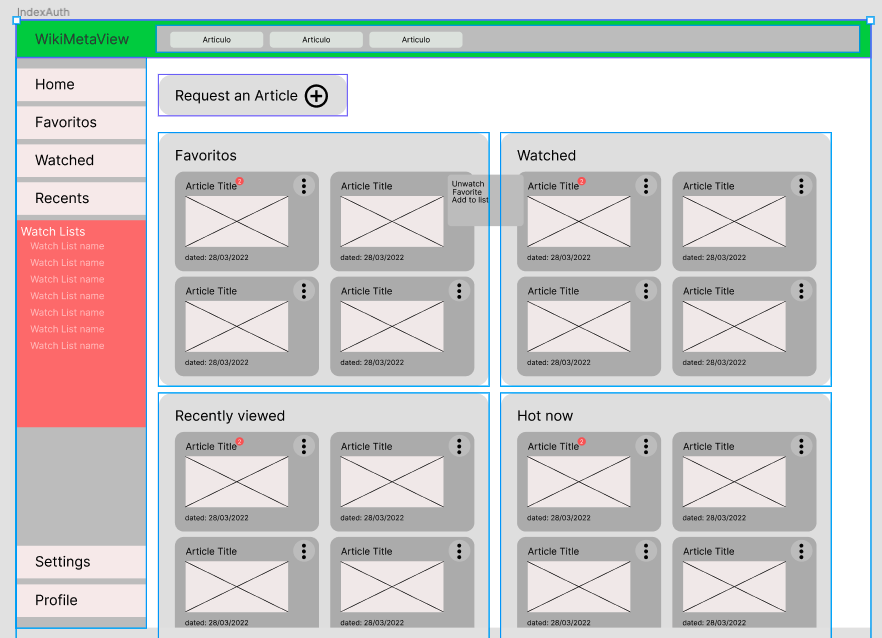
\includegraphics{prototipos/home.png}
\end{figure}



1. Watched
    Muestra una lista y un pequeño abstracto de los artículos que el usuario hace watching y tienen una visualización actualizada

2. Queue
    Muestra una lista de los artículos que le usuario solicito para hacer una visualización pero que el server no ha podido solicitar

3. Explore
    3.1. Favoritos
    Muestra una lista de aquellas visualizaciones que tienen mucha actividad 

    3.2 Watched
    
    3.3. Controversial
    Muestra una lista de aquellas visualizaciones que provocan discusion en la comunidad, caracterizado por muchos comentarios

    3.4 Recientemente vistos

    3.5 Hot now


/index
Esta pagina se encarga de explicar las motivaciones de la App y dar una noción básica del funcionamiento para los watchers.
Tiene el objetivo de cap


/settings



\url{/article?title=<title>&url=<url>}
Muestra un articulo junto con su metadata y las visualizaciones creadas por los usuarios.d



/about
Breve resumen del proyecto, incluye el documento de tesis y documento de seminario asi como datos de contacto y repositorios de github para futuros contribuyentes.

Modales

Query Params Globales

?auth

Si este parámetro esta en el url. Presenta la modal de autenticacion 

?

